\chapter{Resultados}
\label{chap:resultados}

\drop{E}{n} este capítulo se realizará un análisis para mostrar el cumplimiento de los objetivos específicos que se propusieron en el Capítulo \ref{chap:objetivos}.

\section{Desarrollo de un dispositivo \textit{hardware} equipado con distintos sensores.}

El primer objetivo específico de este proyecto era el diseño y desarrollo de un dispositivo \textit{hardware}, que equipase varios sensores necesarios para monitorizar un grupo de expedición. En la Figura \ref{fig:arduino-data} se puede observar cómo el microcontrolador capta los datos de los sensores que equipa, que serán enviados al dispositivo móvil a través del módulo \textit{Bluetooth} conectado al dispositivo.

En las Figuras \ref{fig:pcb_final} y \ref{fig:prototype} se puede observar la \ac{PCB} que ha sido diseñada especialmente para este proyecto y todos los componentes soldados en esta placa.

\begin{figure}[!h]
\begin{center}
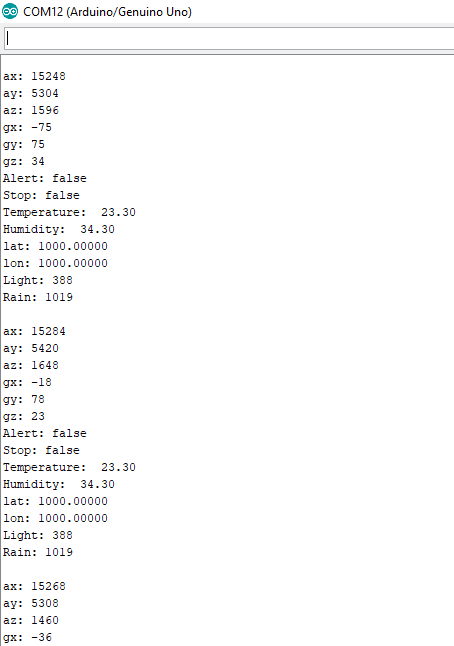
\includegraphics[width=0.75\textwidth]{arduino-data.png}
\caption{Datos de los sensores equipados en el microcontrolador \texttt{Arduino}.}
\label{fig:arduino-data}
\end{center}
\end{figure}

\section{Desarrollo de una aplicación móvil.}

Se puede observar el cumplimiento del objetivo de diseño y desarrollo de una aplicación móvil que recibe datos del microcontrolador a partir del protocolo \textit{Bluetooth} en las Figuras \ref{fig:fig1}, \ref{fig:fig2} y \ref{fig:fig3} de la Sección \ref{functionalityAppMovil}, en las que se aprecian las distintas pantallas que conforman la aplicación móvil, con información relevante tanto para los participantes como para el guía de la expedición. La mayor parte de la información se capta a través de \textit{Bluetooth}, proveniente de los sensores del microcontrolador. La aplicación móvil cumple con toda la funcionalidad que se esperaba desde el comienzo de este proyecto.

\section{Detección inteligente de situaciones anómalas en una expedición.}

Uno de los objetivos principales era el análisis inteligente y en tiempo real de los datos que se captan a través de los sensores que el microcontrolador equipa. Este objetivo engloba tres subobjetivos:

\begin{itemize}
\item \textbf{Detección de caídas.}
\item \textbf{Análisis del grado de dispersión del grupo de expedición.}
\item \textbf{Análisis del riesgo de caída.}
\end{itemize}

A continuación se muestran los resultados que demuestran el cumplimiento de los subobjetivos anteriores:

\subsection{Cumplimiento del objetivo de detección de caídas.}

La detección de caídas parecía ser un objetivo muy factible al inicio del proyecto, utilizando los datos de aceleración lineal y velocidad angular. Pronto se eliminaron los datos de velocidad angular del algoritmo de detección de caídas ya que el dispositivo físico iba a ser portado en la muñeca o en el brazo del usuario de la expedición y los datos de velocidad angular con el microcontrolador en esa situación no eran de utilidad porque el usuario durante una caída puede mover el brazo y la mano de distintas formas.

Por tanto, el algoritmo de detección de caídas de este proyecto está muy limitado debido a que solo infiere la caída basándose en los datos de aceleración lineal. Además, el procesamiento de los datos de aceleración para inferir las caídas son realizados por la aplicación móvil, a partir de datos que recibe por \textit{Bluetooth} desde el microcontrolador. Este hecho se trata de otra limitación, ya que la frecuencia de captación de datos del sensor por parte del microcontrolador es mayor que la frecuencia de envío de los datos por \textit{Bluetooth}, es decir, se leen más datos del sensor de los que se envían por \textit{Bluetooth}. Al ser \textit{Bluetooth} un protocolo inalámbrico, la aplicación móvil en ocasiones recibe datos corruptos, que tiene que descartar, por lo que existen más pérdidas de valores leídos (cabe destacar que el número de paquetes corruptos es muy bajo, pero es necesario comentar que existe dicha situación).

Como última situación desfavorable hay que señalar que la aplicación móvil (como se ha comentado en el capítulo anterior) crea un nuevo hilo por cada paquete de datos que recibe por medio de \textit{Bluetooth}. Esta medida es necesaria, para que la frecuencia de recepción de datos del \textit{socket Bluetooth} sea mayor y pueda realizarse el algoritmo de detección de caídas. Sin embargo, se pueden dar situaciones en las que un paquete con datos de aceleración lineal de un instante posterior sea procesado antes que un paquete con datos de un instante anterior (debido al planificador del sistema operativo del dispositivo móvil). Se podría, por tanto, dar una situación en la que se reciban datos de normalidad (de instantes anteriores) después de procesar datos de caída libre (de instantes posteriores) y la detección de una posible caída fallaría. Esta situación ha sido contemplada y se ha mitigado (como se explicó en el capítulo anterior) aunque es una posible fuente de errores porque no se conoce con certeza cuándo se ejecutará un hilo.

Para medir la precisión del detector de caídas se han realizado un total de cinco caídas de distintas maneras:

\begin{itemize}
\item Caída hacia delante.
\item Caída hacia detrás.
\item Caída lateral.
\end{itemize}

Además, aunque en este proyecto se pensó que el dispositivo físico debería estar situado en la muñeca del usuario de la expedición, se han realizado las mismas pruebas con el dispositivo situado en la cintura. Se ha hecho de esta forma porque un usuario durante una caída puede realizar movimientos del brazo y la muñeca que proporcionen valores de aceleración lineal que no tengan que ver con una caída, por lo que el algoritmo de detección de caídas basado en límites en la aceleración lineal no inferiría una caída.

Los resultados de las pruebas se pueden observar en la Tabla \ref{table:caidas-precision}. Solo un \textbf{33.33\% de todas las caídas fueron detectadas}, cuando el dispositivo era portado en la muñeca del usuario. Si el dispositivo era portado en la cintura del usuario, este porcentaje \textbf{subía hasta el 66.66\%}. El tipo de caída que fue detectado con mayor éxito fue la caída hacia detrás, ya que la forma en la que se cae se asemeja más a la ideal. Además, en este tipo de caída los brazos suelen acompañar al movimiento que hace el cuerpo al contrario que en la caída hacia delante en la que los brazos realizan movimientos más bruscos (para intentar plantar las manos en el suelo y minimizar los daños que la caída pudiese producir) que conllevan variaciones en la aceleración lineal y desviaciones con respecto a la caída ideal.

El dispositivo se ha probado en situaciones reales, durante expediciones en la naturaleza de distinta dificultad y en distintos terrenos como el asfalto, pistas de tierra y senderos con mucha piedra y desnivel. No se ha detectado ninguna caída realizando dichas expediciones por lo que se han producido un \textbf{0\% de falsos positivos}. Esto mejora mucho los resultados del detector de caídas ya que si el guía recibe una alerta de caída puede estar casi convencido de que se trata de una alerta real y no un falso positivo. 

Cabe desatacar también que el microcontrolador está equipado con dos botones físicos y uno de ellos genera una alerta por caída. De esta forma, si un usuario se encuentra consciente después de una caída puede pulsar este botón del dispositivo para generar la alerta por caída.

\begin{table}[!h]
\centering
\begin{tabular}{l|c|c|}
\cline{2-3}
                                                                                                  & \multicolumn{1}{l|}{\cellcolor[HTML]{656565}{\color[HTML]{FFFFFF} \textbf{\begin{tabular}[c]{@{}l@{}}Caídas detectadas con el\\ dispositivo en la muñeca\end{tabular}}}} & \multicolumn{1}{l|}{\cellcolor[HTML]{656565}{\color[HTML]{FFFFFF} \textbf{\begin{tabular}[c]{@{}l@{}}Caídas detectadas con el\\ dispositivo en la cintura\end{tabular}}}} \\ \hline
\rowcolor[HTML]{EFEFEF} 
\multicolumn{1}{|l|}{\cellcolor[HTML]{EFEFEF}{\color[HTML]{000000} \textbf{Caída hacia delante}}} & {\color[HTML]{000000} 1 de 5}                                                                                                                                            & {\color[HTML]{000000} 3 de 5}                                                                                                                                             \\ \hline
\multicolumn{1}{|l|}{{\color[HTML]{000000} \textbf{Caída hacia detrás}}}                          & {\color[HTML]{000000} 3 de 5}                                                                                                                                            & {\color[HTML]{000000} 4 de 5}                                                                                                                                             \\ \hline
\rowcolor[HTML]{EFEFEF} 
\multicolumn{1}{|l|}{\cellcolor[HTML]{EFEFEF}{\color[HTML]{000000} \textbf{Caída lateral}}}       & {\color[HTML]{000000} 2 de 5}                                                                                                                                            & {\color[HTML]{000000} 3 de 5}                                                                                                                                             \\ \hline
\end{tabular}
\caption{Precisión del algoritmo de detección de caídas, ante distintas pruebas.}
\label{table:caidas-precision}
\end{table}

\subsection{Cumplimiento del objetivo de análisis del grado de dispersión en el grupo de expedición.}

Para demostrar el correcto funcionamiento del algoritmo de análisis del grado de dispersión del grupo de expedición, se va a plantear una situación hipotética en la que existen un total de cuatro usuarios (un guía y tres participantes). Se compararán los resultados obtenidos por el algoritmo desarrollado en el presente proyecto, los resultados obtenidos por \texttt{Google Maps} y los obtenidos de forma manual. Los usuarios se encuentran en la ciudad de Ciudad Real (como se puede observar en la Figura \ref{fig:google-location}).

Las coordenadas de los usuarios de esta expedición se pueden encontrar en la Tabla \ref{table:situation-hipotetica}.

\begin{table}[!h]
\centering
\begin{tabular}{lcccc}
\rowcolor[HTML]{656565} 
\multicolumn{1}{c}{\cellcolor[HTML]{656565}{\color[HTML]{FFFFFF} \textbf{Usuario}}} & {\color[HTML]{FFFFFF} \textbf{\begin{tabular}[c]{@{}c@{}}Latitud en\\ grados\end{tabular}}} & {\color[HTML]{FFFFFF} \textbf{\begin{tabular}[c]{@{}c@{}}Longitud\\ en grados\end{tabular}}} & {\color[HTML]{FFFFFF} \textbf{\begin{tabular}[c]{@{}c@{}}Latitud en\\ radianes\end{tabular}}} & {\color[HTML]{FFFFFF} \textbf{\begin{tabular}[c]{@{}c@{}}Longitud\\ en radianes\end{tabular}}} \\
{\color[HTML]{000000} Guía}                                                         & {\color[HTML]{000000} 38.989}                                                               & {\color[HTML]{000000} -3.929}                                                                & {\color[HTML]{000000} 0.680486}                                                               & {\color[HTML]{000000} -0.06857}                                                                \\
\rowcolor[HTML]{EFEFEF} 
{\color[HTML]{000000} Participante 1}                                               & {\color[HTML]{000000} 38.981}                                                               & {\color[HTML]{000000} -3.925}                                                                & {\color[HTML]{000000} 0.6803467}                                                              & {\color[HTML]{000000} -0.068504}                                                               \\
{\color[HTML]{000000} Participante 2}                                               & {\color[HTML]{000000} 38.982}                                                               & {\color[HTML]{000000} -3.930}                                                                & {\color[HTML]{000000} 0.6803642}                                                              & {\color[HTML]{000000} -0.068591}                                                               \\
\rowcolor[HTML]{EFEFEF} 
{\color[HTML]{000000} Participante 3}                                               & {\color[HTML]{000000} 38.980}                                                               & {\color[HTML]{000000} -3.934}                                                                & {\color[HTML]{000000} 0.6803293}                                                              & {\color[HTML]{000000} -0.68661}                                                               
\end{tabular}
\caption{Coordenadas en grados y en radianes de los usuarios de la expedición hipotética planteada.}
\label{table:situation-hipotetica}
\end{table}

Se han usado dichos valores de entrada en el algoritmo implementado en este proyecto (véase Listado \ref{lst:hipotetica}) para obtener el grado de dispersión del grupo. Los resultados de salida del algoritmo se pueden observar en la Figura \ref{fig:exit-dispersion}.

\begin{lstlisting}[language=java,captionpos=t,caption={\textbf{Test de análisis del grado de dispersión en una situación hipotética planteada.}},label={lst:hipotetica}]
public void TestDispersionGrupo() {
  double lat_guide = 38.989; double lon_guide = -3.929;
  double lat_p1 = 38.981; double lon_p1 = -3.925;
  double lat_p2 = 38.982; double lon_p2 = -3.930;
  double lat_p3 = 38.980; double lon_p3 = -3.934;

  double d1 = getDistanceBetweenTwoPoints(Math.toRadians(lat_guide), Math.toRadians(lon_guide),
            Math.toRadians(lat_p1), Math.toRadians(lon_p1));
  double d2 = getDistanceBetweenTwoPoints(Math.toRadians(lat_guide), Math.toRadians(lon_guide),
            Math.toRadians(lat_p2), Math.toRadians(lon_p2));
  double d3 = getDistanceBetweenTwoPoints(Math.toRadians(lat_guide), Math.toRadians(lon_guide),
            Math.toRadians(lat_p3), Math.toRadians(lon_p3));

  double dispersion = (0.333333333) * (d1+d2+d3);

  Log.d("GVIDI", "Distancia entre guía y participante 1 = " + String.valueOf(d1));
  Log.d("GVIDI", "Distancia entre guía y participante 2 = " + String.valueOf(d2));
  Log.d("GVIDI", "Distancia entre guía y participante 3 = " + String.valueOf(d3));
  Log.d("GVIDI", "Dispersión del grupo = " + String.valueOf(dispersion));
}
\end{lstlisting}

\begin{figure}[!h]
\begin{center}
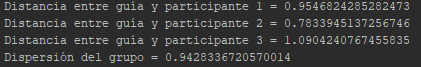
\includegraphics[width=0.75\textwidth]{resultados-dispersion.png}
\caption{Salida del algoritmo que calcula el grado de dispersión de la expedición, para una situación hipotética planteada.}
\label{fig:exit-dispersion}
\end{center}
\end{figure}

Las distancias que calcula \texttt{Google Maps} se pueden observar en la figura \ref{fig:google-location}.

\begin{figure}[!h]
\begin{center}
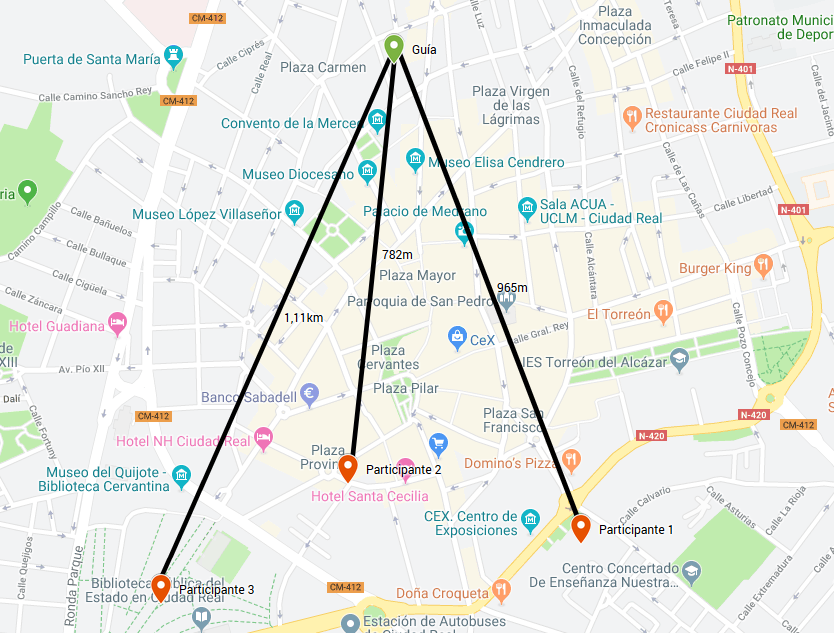
\includegraphics[width=0.75\textwidth]{result-google-maps.png}
\caption{Localización de los usuarios de la expedición hipotética planteada.}
\label{fig:google-location}
\end{center}
\end{figure}

Las distancias calculadas de forma manual, usando la fórmula de \textit{Harvesine} (que se encuentra en la Sección \ref{MapaRecorrido}) son las siguientes:

distancia(guía, participante1) = $2\cdot 6373 \cdot \arcsin \left( \sqrt{\sin^2 \left( \frac{0.6803467 - 0.680486}{2} \right) +$ \\ $+ \cos \left(0.680486\right) \cdot \cos \left(0.6803467\right) \cdot \sin^2 \left( \frac{-0.068504 + 0.06857}{2} \right)} \right) \approx 1.10$ \\


distancia(guía, participante2) = $2\cdot 6373 \cdot \arcsin \left( \sqrt{\sin^2 \left( \frac{0.6803642 - 0.680486}{2} \right) +$ \\ $+ \cos \left(0.680486\right) \cdot \cos \left(0.6803642\right) \cdot \sin^2 \left( \frac{-0.068591 + 0.06857}{2} \right)} \right) \approx 0.797$ \\


distancia(guía, participante3) = $2\cdot 6373 \cdot \arcsin \left( \sqrt{\sin^2 \left( \frac{0.6803293 - 0.680486}{2} \right) +$ \\ $+ \cos \left(0.680486\right) \cdot \cos \left(0.6803293\right) \cdot \sin^2 \left( \frac{-0.068661 + 0.06857}{2} \right)} \right) \approx 1.32$

En la Tabla \ref{comparativa-separacion} se puede observar la comparativa entre los distintos grados de separación obtenidos en esta expedición hipotética usando el algoritmo desarrollado en este proyecto, la plataforma \texttt{Google Maps} y aplicando la fórmula descrita en la Sección \ref{MapaRecorrido}. Se puede observar que los resultados del algoritmo propuesto y de \texttt{Google Maps} son prácticamente idénticos. La desviación existente con el cálculo manual radica principalmente en la precisión de los decimales que se usan, ya que las operaciones trigonométricas utilizadas (seno, arcoseno y coseno) son muy sensibles a cambios en los decimales.

\begin{table}[!h]
\centering
\begin{tabular}{l|c|c|c|}
\cline{2-4}                                                                                                & \multicolumn{1}{c|}{\cellcolor[HTML]{656565}{\color[HTML]{FFFFFF} \textbf{\begin{tabular}[c]{@{}c@{}}Algoritmo del\\ proyecto\end{tabular}}}} & \multicolumn{1}{c|}{\cellcolor[HTML]{656565}{\color[HTML]{FFFFFF} \textbf{De forma manual}}} & \multicolumn{1}{c|}{\cellcolor[HTML]{656565}{\color[HTML]{FFFFFF} \textbf{\texttt{Google Maps}}}} \\ \hline
\rowcolor[HTML]{EFEFEF} 
\multicolumn{1}{|l|}{\cellcolor[HTML]{EFEFEF}{\color[HTML]{000000} Distancia(guía, participante1)}} & {\color[HTML]{000000} 0.955km}                                                                                                                & {\color[HTML]{000000} 1.1km}                                                                 & {\color[HTML]{000000} 0.965km}                                                                    \\ \hline
\multicolumn{1}{|l|}{{\color[HTML]{000000} Distancia(guía, participante2)}}                         & {\color[HTML]{000000} 0.783km}                                                                                                                & {\color[HTML]{000000} 0.797km}                                                               & {\color[HTML]{000000} 0.782km}                                                                    \\ \hline
\rowcolor[HTML]{EFEFEF} 
\multicolumn{1}{|l|}{\cellcolor[HTML]{EFEFEF}{\color[HTML]{000000} Distancia(guía, participante3)}} & {\color[HTML]{000000} 1.09km}                                                                                                                 & {\color[HTML]{000000} 1.32km}                                                                & {\color[HTML]{000000} 1.11km}                                                                     \\ \hline
\multicolumn{1}{|l|}{{\color[HTML]{000000} Grado de separación}}                                    & {\color[HTML]{000000} 0.943km}                                                                                                                & {\color[HTML]{000000} 1.072km}                                                               & {\color[HTML]{000000} 0.952km}                                                                    \\ \hline
\end{tabular}
\caption{Comparativa del grado de separación obtenido de diversas maneras.}
\label{comparativa-separacion}
\end{table}

\subsection{Cumplimiento del objetivo de análisis del riesgo de caída.}

Al igual que en el apartado anterior, se van a realizar un total de tres \textit{tests} para demostrar que la salida del algoritmo de análisis del riesgo de caída, basado en el empleo de lógica difusa, es la esperada para unos ciertos valores de entrada. Cabe recordar que las variables de entrada de este algoritmo son:

\begin{itemize}
\item La humedad que existe en la expedición.
\item La presencia o ausencia de lluvia.
\item La cantidad de luz que hay en un momento dado en la expedición. 
\end{itemize}

Como única variable de salida se encuentra el riesgo de caída en un preciso instante.

\subsubsection{\textit{Test} 1.}

En la Tabla \ref{table:test1} se encuentran los valores que tomarán las distintas variables de entrada en el \textit{Test} 1. También se puede observar a qué conjunto difuso pertenecen dichos valores.

\begin{table}[!h]
\centering
\begin{tabular}{l|c|c|c|}
\cline{2-4}
                                                                                    & \cellcolor[HTML]{656565}{\color[HTML]{FFFFFF} \textbf{Humedad}} & \cellcolor[HTML]{656565}{\color[HTML]{FFFFFF} \textbf{Lluvia}} & \cellcolor[HTML]{656565}{\color[HTML]{FFFFFF} \textbf{Luz}} \\ \hline
\rowcolor[HTML]{EFEFEF} 
\multicolumn{1}{|l|}{\cellcolor[HTML]{EFEFEF}{\color[HTML]{000000} \textbf{Valor}}} & {\color[HTML]{000000} 90\%}                                      & {\color[HTML]{000000} 200}                                     & {\color[HTML]{000000} 250}                                  \\ \hline
\multicolumn{1}{|l|}{{\color[HTML]{000000} \textbf{Conjunto difuso}}}               & {\color[HTML]{000000} Muy alta}                                 & {\color[HTML]{000000} Sí}                                      & {\color[HTML]{000000} Oscuro}                               \\ \hline
\end{tabular}
\caption{Valores y conjuntos difusos de las variables de entrada del \textit{Test} 1.}
\label{table:test1}
\end{table}

Para este primer \textit{test}, se activaría la siguiente regla (del conjunto de reglas definidas en este proyecto, que se pueden consultar en la Sección \ref{analysis_risk}:

\begin{itemize}
\item \textbf{R4.} Si lluvia es sí $\wedge$ (luz es oscuro $\vee$ luz es muy oscuro) $\rightarrow$ riesgo es \textbf{alto}
\end{itemize}

Si la cantidad de luz que hay en un momento determinado es baja, aumenta la dificultad para ver obstáculos en el camino y por tanto aumenta también el riesgo de caída. Si además está lloviendo, el terreno puede estar resbaladizo por lo que el riesgo de caída también aumenta. Ante una situación con una visibilidad baja y lluvia el riesgo de caída debe ser alto. Por lo tanto, la salida del algoritmo difuso para este \textit{test} debería ser un riesgo alto de caída.

La detección del riesgo de caída se realiza usando únicamente tres variables de entrada por limitaciones económicas. Sin embargo este enfoque usando lógica difusa hace que sea muy sencillo añadir nuevos sensores que ayuden a realizar un análisis del riesgo de caída en un futuro, como pueden ser aquellos relacionados con la pendiente y dificultad del terreno.

\subsubsection{\textit{Test} 2.}

En la Tabla \ref{table:test2} se encuentran los valores que tomarán las distintas variables de entrada en el \textit{Test} 2. También se puede observar a qué conjunto difuso pertenecen dichos valores.

\begin{table}[!h]
\centering
\begin{tabular}{l|c|c|c|}
\cline{2-4}
                                                                                    & \cellcolor[HTML]{656565}{\color[HTML]{FFFFFF} \textbf{Humedad}} & \cellcolor[HTML]{656565}{\color[HTML]{FFFFFF} \textbf{Lluvia}} & \cellcolor[HTML]{656565}{\color[HTML]{FFFFFF} \textbf{Luz}} \\ \hline
\rowcolor[HTML]{EFEFEF} 
\multicolumn{1}{|l|}{\cellcolor[HTML]{EFEFEF}{\color[HTML]{000000} \textbf{Valor}}} & {\color[HTML]{000000} 40\%}                                     & {\color[HTML]{000000} 512}                                     & {\color[HTML]{000000} 700}                                  \\ \hline
\multicolumn{1}{|l|}{{\color[HTML]{000000} \textbf{Conjunto difuso}}}               & {\color[HTML]{000000} Media}                                    & {\color[HTML]{000000} 50\% Sí, 50\% No}                        & {\color[HTML]{000000} Día}                                  \\ \hline
\end{tabular}
\caption{Valores y conjuntos difusos de las variables de entrada del \textit{Test} 2.}
\label{table:test2}
\end{table}

En este segundo \textit{test}, se activarán las siguientes reglas:

\begin{itemize}
\item \textbf{R1.} Si lluvia es sí $\wedge$ (luz es media-alta $\vee$ luz es máxima) $\wedge$ (humedad es muy baja $\vee$ humedad es baja $\vee$ humedad es media) $\rightarrow$ riesgo es \textbf{bajo} 

\item \textbf{R6.} Si lluvia es no $\wedge$ (luz es media-alta $\vee$ luz es máxima) $\rightarrow$ riesgo es \textbf{bajo}
\end{itemize}

En este caso en vez de activarse tan sólo una regla se activan un total de dos reglas, ya que existe un 50\% de posibilidades de que esté lloviendo. En este proyecto, se usa el producto algebraico como método de conjunción entre reglas. Esto es, las distintas funciones de pertenencia a los conjuntos difusos se multiplican por el grado de cumplimiento de la condición y por último se combinan. En este caso, como la salida de ambas reglas es un riesgo bajo, el resultado del algoritmo debería ser un riesgo bajo de caída.

En esta situación es lógico el valor del riesgo bajo de caída porque independientemente de si llueve o no, la cantidad de luz que existe es suficiente para detectar posibles obstáculos en el camino y la humedad es aceptable para un riesgo de caída bajo.

\subsubsection{\textit{Test} 3.}

En la Tabla \ref{table:test3} se encuentran los valores que tomarán las distintas variables de entrada en el \textit{Test} 3. También se puede observar a qué conjunto difuso pertenecen dichos valores.

\begin{table}[!h]
\centering
\begin{tabular}{l|c|c|c|}
\cline{2-4}
                                                                                    & \cellcolor[HTML]{656565}{\color[HTML]{FFFFFF} \textbf{Humedad}} & \cellcolor[HTML]{656565}{\color[HTML]{FFFFFF} \textbf{Lluvia}} & \cellcolor[HTML]{656565}{\color[HTML]{FFFFFF} \textbf{Luz}} \\ \hline
\rowcolor[HTML]{EFEFEF} 
\multicolumn{1}{|l|}{\cellcolor[HTML]{EFEFEF}{\color[HTML]{000000} \textbf{Valor}}} & {\color[HTML]{000000} 90\%}                                     & {\color[HTML]{000000} 100}                                     & {\color[HTML]{000000} 1000}                                 \\ \hline
\multicolumn{1}{|l|}{{\color[HTML]{000000} \textbf{Conjunto difuso}}}               & {\color[HTML]{000000} Muy alta}                                 & {\color[HTML]{000000} Sí}                                      & {\color[HTML]{000000} Mucha luz}                            \\ \hline
\end{tabular}
\caption{Valores y conjuntos difusos de las variables de entrada del \textit{Test} 3.}
\label{table:test3}
\end{table}

Para este último \textit{test}, se activaría la siguiente regla:

\begin{itemize}
\item \textbf{R2.} Si lluvia es sí $\wedge$ (luz es media-alta $\vee$ luz es máxima) $\wedge$ (humedad es alta $\vee$ humedad muy alta) $\rightarrow$ riesgo es \textbf{medio}
\end{itemize}

En este caso, además de estar lloviendo la humedad es alta. Este hecho aumenta el riesgo de caída porque la estabilidad el terreno puede no ser la idónea. Sin embargo, como las condiciones de iluminación exterior son correctas, el riesgo de caída no llega a ser alto. Por lo tanto, la salida del algoritmo difuso para este \textit{test} debería ser un riesgo medio de caída.

\subsubsection{Resultados del algoritmo de análisis del riesgo de caída.}

En el Listado \ref{lst:hipotetica-riesgo} se puede observar el código empleado para llevar a cabo los \textit{tests} propuestos anteriormente.

\begin{lstlisting}[language=java,captionpos=t,caption={\textbf{Cálculo del riesgo de caída en una expedición, para unos valores de humedad, luz y lluvia dados.}},label={lst:hipotetica-riesgo}]
public void TestAnalisisRiesgo() {
  FuzzyRiskAnalysis.Build();
  // Los parámetros del método CalculateRisk son (humedad, lluvia, luz)
  String value = FuzzyRiskAnalysis.CalculateRisk(90.0, 200.0, 250.0);
  printResult(1, value);
  value = FuzzyRiskAnalysis.CalculateRisk(40.0, 512.0, 700.0);
  printResult(2, value);
  value = FuzzyRiskAnalysis.CalculateRisk(90.0, 100.0, 1000.0);
  printResult(3, value);
}
\end{lstlisting}

La salida del algoritmo que calcula el riesgo de caída en la expedición para los \textit{test} propuestos anteriormente se puede ver en la Figura \ref{fig:salida-riesgo}.

\begin{figure}[!h]
\begin{center}
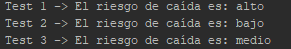
\includegraphics[width=0.75\textwidth]{salida-riesgo.png}
\caption{Salida del algoritmo que calcula el riesgo de caída en la expedición, para los \textit{tests} aquí propuestos.}
\label{fig:salida-riesgo}
\end{center}
\end{figure}

\section{Desarrollo de una plataforma web}

En este proyecto se ha desarrollado una plataforma \textit{web} que permite a los usuarios (y a familiares y amigos si los usuarios lo permiten) visualizar información sobre la expedición que están realizando en tiempo real. Esta información ha sido procesada y almacenada en una base de datos \textit{cloud} por parte de la aplicación móvil ya comentada. 

En las Figuras \ref{fig:signinWeb}, \ref{fig:todasRutas}, \ref{fig:infogeneral} y \ref{fig:mapainfo} de la Sección \ref{platformweb} se puede observar la interfaz de usuario de la plataforma \textit{web}, vista desde un ordenador portátil con un tamaño de pantalla de $15.6$ pulgadas. La \textit{web} tiene un diseño \textit{responsive}, ya que se adapta a distintos dispositivos con tamaños de pantalla diferentes. Esto se puede observar en las Figuras \ref{fig:fig1mobile} y \ref{fig:fig2mobile} en las que se ve la interfaz gráfica adaptada a la pantalla de un \texttt{iPhone X}, de $5.8$ pulgadas. En este caso, también se han cumplido con todos los objetivos propuestos al inicio del proyecto.

No solo es posible visualizar una expedición en tiempo real sino que también se pueden analizar expediciones realizadas anteriormente, como se puede observar en la Figura \ref{fig:todasRutas}.

\begin{figure}
 \centering
  \subfloat[Página de inicio de sesión de la aplicación \textit{web}, vista desde un dispositivo móvil.]{
   \label{fig:loginmobile}
    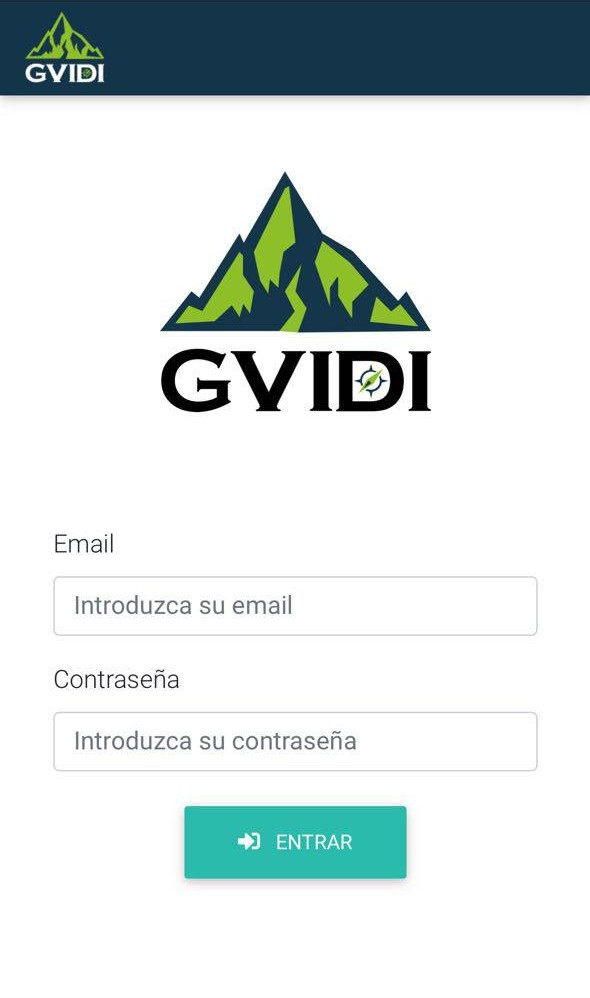
\includegraphics[width=0.45\textwidth]{login-mobile.jpg}}
  \subfloat[Página que contiene el histórico de rutas de un usuario, vista desde un dispositivo móvil.]{
   \label{fig:rutasmobile}
    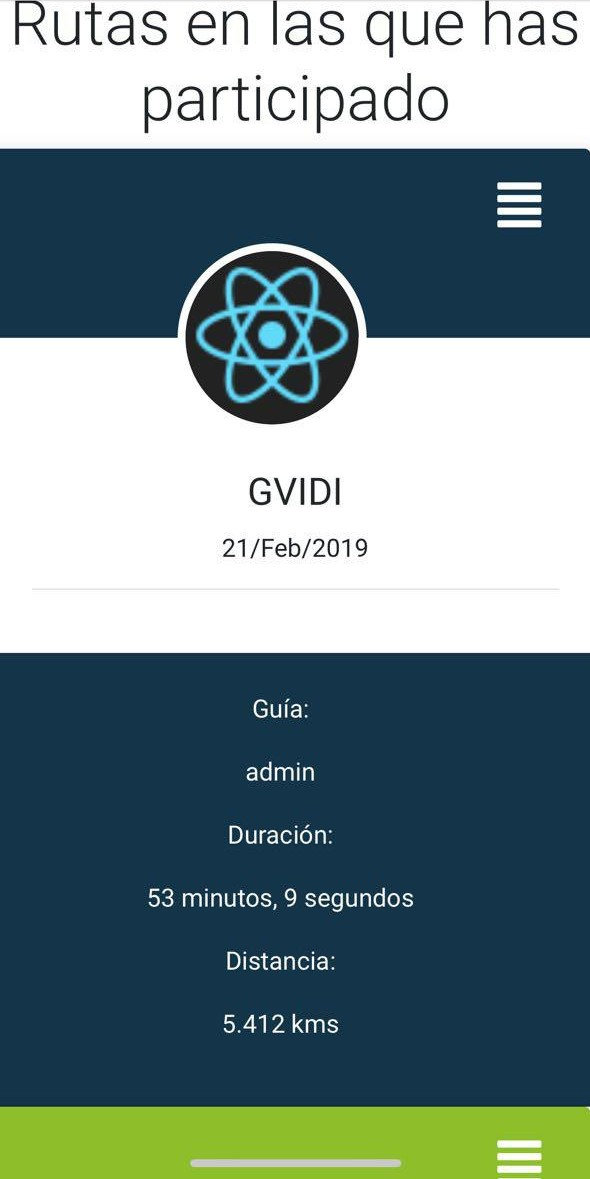
\includegraphics[width=0.45\textwidth]{rutas-mobile.jpg}}
    
  \caption{Páginas de \textit{login} e histórico de rutas desde un dispositivo móvil \texttt{iPhone X}}
  \label{fig:fig1mobile}
\end{figure}

\begin{figure}[!h]
\begin{center}
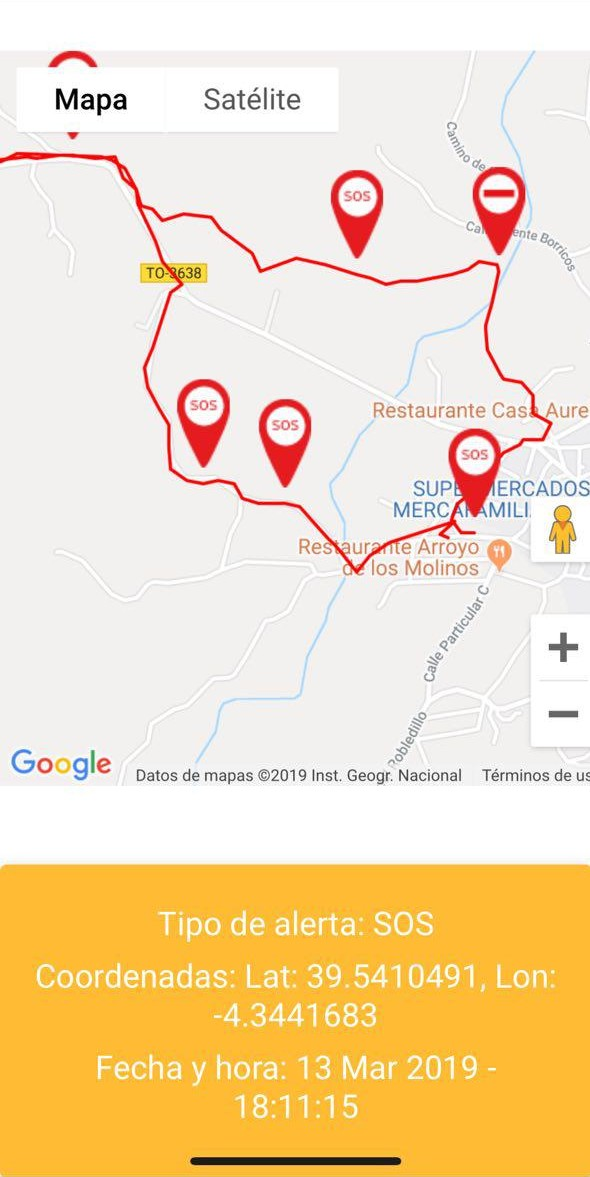
\includegraphics[width=0.5\textwidth]{especifica-mobile.jpg}
\caption{Página de información específica acerca de una expedición, vista desde un dispositivo móvil.}
\label{fig:fig2mobile}
\end{center}
\end{figure}

\section{Competencias específicas de intensificación trabajadas durante este proyecto}
\label{competencias-inten}

A lo largo de este proyecto se han trabajado competencias específicas de la intensificación que he cursado: \textbf{Ingeniería de Computadores}. Estas competencias son las siguientes:

\begin{itemize}
\item \textbf{Capacidad de diseñar y construir sistemas digitales, incluyendo computadores, sistemas basados en microprocesador y sistemas de comunicaciones.} En este proyecto se ha desarrollado un dispositivo \textit{hardware} consistente en un microcontrolador \texttt{Arduino} equipado con una serie de sensores. Además, se ha diseñado una \ac{PCB} para eliminar el uso de cables de prototipado y crear un dispositivo con un aspecto más profesional. La comunicación entre el microcontrolador y la aplicación móvil desarrollada se lleva a cabo usando el protocolo de comunicaciones inalámbrico \textit{Bluetooth}.

\item \textbf{Capacidad de desarrollar procesadores específicos y sistemas empotrados, así como desarrollar y optimizar el \textit{software} de dichos sistemas.} Durante este \ac{TFG} se ha desarrollado \textit{software} específico para interaccionar con el dispositivo físico desarrollado. Este \textit{software} incluye tanto el código fuente que es ejecutado directamente por el microcontrolador como las librerías que se han usado para captar datos de los sensores equipados en el dispositivo.

\item \textbf{Capacidad de analizar y evaluar arquitecturas de computadores, incluyendo plataformas paralelas y distribuidas, así como desarrollar y optimizar \textit{software} para las mismas.} En este proyecto se ha planteado una arquitectura distribuida entre los distintos dispositivos físicos que portan los usuarios de la expedición, la aplicación móvil desarrollada que se encuentra instalada en los dispositivos móviles de los usuarios y la plataforma \textit{web} que permite la visualización tanto en tiempo real como de forma histórica de los datos relativos con la expedición.

\item \textbf{Capacidad de diseñar e implementar \textit{software} de sistema y de comunicaciones.} Se ha desarrollado \textit{software} específico para tratar con algunos de los sensores que el dispositivo equipa. De igual forma, se ha desarrollado \textit{software} que permite la comunicación usando el protocolo \textit{Bluetooth} entre el dispositivo móvil y el microcontrolador. La comunicación de datos entre la aplicación móvil y la plataforma \textit{web} se realiza a través de una base de datos \textit{cloud} \texttt{NoSQL}. La aplicación móvil almacena en la base de datos la información procesada en tiempo real y la plataforma \textit{web} realiza consultas a la misma para obtener los datos almacenados y mostrarlos al usuario.

\item \textbf{Capacidad de analizar, evaluar y seleccionar las plataformas \textit{hardware} y \textit{software} más adecuadas para el soporte de aplicaciones empotradas y de tiempo real.} Como se puede observar en el Anexo \ref{chap:antecedentes}, se han analizado y evaluado distintas plataformas \textit{hardware} para desarrollar el dispositivo físico que se expone en este proyecto. También se han analizado las alternativas existentes a los sensores usados en este proyecto y se han seleccionado aquellos con una mejor relación calidad-precio.  De igual forma, se han tomado decisiones que contemplan distintas alternativas en cuanto a las plataformas \textit{software}. Una de estas decisiones es el uso de \textit{Android} como sistema operativo para la aplicación móvil frente al desarrollo de una aplicación móvil para el sistema operativo \texttt{iOS}. También se han evaluado distintas plataformas \textit{software} para el desarrollo de la plataforma \textit{web}. Finalmente se ha usado una arquitectura cliente-servidor, con \texttt{node} en el lado del servidor y \texttt{react} en el lado del cliente.

\item \textbf{Capacidad para analizar, evaluar, seleccionar y configurar plataformas hardware para el desarrollo y ejecución de aplicaciones y servicios informáticos.} Para la consecución de este proyecto se han contemplado distintas alternativas, como se puede observar en el Anexo \ref{chap:antecedentes}. Entre estas alternativas destacan la \texttt{Rasbperry Pi} y la familia de circuitos integrados \texttt{STM32}. Finalmente se decidió usar la plataforma \texttt{Arduino} (como se comenta en la sección indicada anteriormente) y se ha desarrollado \textit{software} para esta plataforma.

\end{itemize}